\subsection*{Основные понятия}

Представьте себе обычную таблицу, где присутсвуют именованные столбцы "--- имена этих столбцов будем называть \textit{признаками}.

\textit{Объектом} будем называть единицу, для которой необходимо совершить предсказание, в контексте таблицы "--- одна строка. Возвращаясь к примеру с квартирами, объектом будет являться одна конкретная квартира. 

Множество всех доступных объектов будем обозначать через~$\mathbb{X}$, целевую переменную (и соответственно, множество всех целевых переменных) — через~$y \in \mathbb{Y}$. Совокупность $(x, y)$ называется \textit{обучающим примером}, а их полное множество — \textit{обучающей выборкой}:
\begin{gather*}
X = {(x_1, y_1), (x_2, y_2), \dots, (x_\ell, y_\ell)} \
X = {(x_i, y_i)}_{i=1}^\ell,
\end{gather*}
где $\ell$ — их количество.

Конечно, мы не можем напрямую дать компьютеру задачу «предскажи цену квартиры», так как компьютер не понимает, что такое квартира, площадь квартиры и так далее. Поэтому необходимо представить объект в виде набора признаков — т.н. \textit{признаковое описание}. Объект $x \in \mathbb{X}$ можно представить вектором $(x_1, x_2, \dots, x_d)$, где $x_i$ — $i$-й признак данного объекта, а $d$ "--- количество признаков. Такие признаки могут быть разными, среди основных выделяют:

\begin{itemize}
\item Числовые: $x_i \in \mathbb{R}$ (например, площадь квартиры, цена);
\item Категориальные: $x_i \in \{c_1, c_2, \dots, c_k\}$, где множество категорий неупорядочено (например, район города);
\item Упорядоченные категориальные: категориальные с чётким порядком (например, оценка по 5-балльной шкале);
\item Множествозначные (\texttt{set-valued}): значение $x_i$ является подмножеством универсального множества (например, хэштеги под видео). Иными словами "--- когда значение признака можно задать с помощью нескольких категориальных признаков;
\item Временные (\texttt{time-based}): признаки, связанные со временем, например, дата покупки, час обращения, год выпуска.
\end{itemize}

\newpage
Как мы обсуждали ранее, мы хотим каждый объект представлять в векторной форме $(x_1, ...,x_d)$. Внимательный читатель мог задаться вопросом "--- а как мы собираемся помещать в вектор нечисловые признаки? Скажем, что если у нас есть категориальный признак в наборе данных?

В таких случаях можно (и нужно) прибегнуть к специальным кодирующим алгоритмам. Так, наиболее популярным алгоритмам для кодирования признаков является \texttt{one-hot-encoding}. Его идея заключается в следующем: пусть у нас есть признак $color$, который является категориальным и принимает значения из множества $\{A, B, C\}$. В результате работы алгоритма, вместо признака $color$ появляются признаки $colorA$, $colorB$,$colorC$, затем присваивается 1 или 0 в соответствии тому значению, которое было ранее у каждого объекта.

\begin{figure}[H]
    \centering
    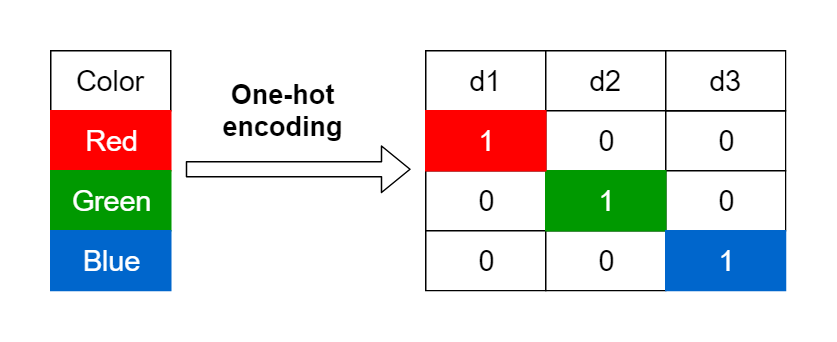
\includegraphics[width=1\linewidth]{media/onehotencoding.png}
\end{figure}

В зависимости от значений, которые принимает $y$, задачи машинного обучения также делятся на:
\begin{itemize}
\item \textbf{Регрессия:} $\mathbb{Y} = \mathbb{R}$ — предсказание числовых значений (например, цена квартиры);
\item \textbf{Бинарная классификация:} $\mathbb{Y} = {0, 1}$ — два возможных класса (например, болезнь есть/нет);
\item \textbf{Многоклассовая классификация:} $\mathbb{Y} = {0, 1, \dots, K}$ — более двух категорий (например, прогноз погоды: «ясно», «облачно», «дождь»);
\end{itemize}